\documentclass[aspectratio=169,11pt]{beamer}

\usetheme{Madrid}
\usecolortheme{seahorse}
\usefonttheme{professionalfonts}
\setbeamertemplate{navigation symbols}{}
\setbeamertemplate{itemize items}[circle]
\setbeamertemplate{enumerate items}[default]

\usepackage[utf8]{inputenc}
\usepackage{amsmath,amssymb,bm}
\usepackage{booktabs}
\usepackage{tikz}
\usetikzlibrary{arrows.meta,positioning,calc,shapes.geometric}
\usepackage{xcolor}
\usepackage{listings}

\definecolor{deepblue}{RGB}{30,64,175}
\definecolor{softblue}{RGB}{219,234,254}
\definecolor{softgreen}{RGB}{220,252,231}
\definecolor{softorange}{RGB}{255,237,213}
\definecolor{softred}{RGB}{254,226,226}
\definecolor{darkgray}{RGB}{55,65,81}

\setbeamercolor{title}{fg=deepblue}
\setbeamercolor{frametitle}{fg=deepblue}
\setbeamercolor{structure}{fg=deepblue}
\setbeamercolor{block title}{bg=deepblue,fg=white}
\setbeamercolor{block body}{bg=softblue,fg=black}

\lstset{
  basicstyle=\ttfamily\scriptsize,
  breaklines=true,
  columns=fullflexible,
  frame=single,
  backgroundcolor=\color{softblue},
  rulecolor=\color{deepblue},
  keywordstyle=\color{deepblue}\bfseries,
  commentstyle=\color{darkgray},
  showstringspaces=false
}

\title[]{
Dupire vs. Neural Networks Delta Hedging}
\subtitle{Erdos Project}
\author[Arevalo, O Cobhthaigh, Hewitt, Zhang]{Oscar Arevalo, Micheal O Cobhthaigh, Alec Hewitt, Ziqing Zhang}
\date{\today}

\begin{document}

%------------------------------------------------
\begin{frame}
  \titlepage
\end{frame}



\begin{frame}{Overview}
\begin{itemize}
    \item Dupire model: Why constant volatility is insufficient and how local volatility uses the implied volatility surface.
    \item Neural network approach: How to hedge using a neural network approach using market features.
    \item Results and comparison: How the Dupire and neural-network hedges perform in the backtest.
\end{itemize}
\end{frame}

\begin{frame}{Motivation: Beyond Black--Scholes}
  \begin{itemize}
    \item Black--Scholes dynamics:
    \[
      dS_t = rS_t\,dt + \sigma S_t\,dW_t .
    \]
    \item However, in reality volatilities vary across strikes and maturities:
    \[
      \sigma_{\mathrm{imp}} = \sigma_{\mathrm{imp}}(K,T).
    \]
    \begin{itemize}
        \item Upshot: a constant volatility breaks down in reality.
    \end{itemize}
    
\item Dupire uses the implied volatility surface to infer a local volatility surface for the underlying asset.
  \end{itemize}
\end{frame}

\begin{frame}{Dupire Local Volatility}
  \begin{itemize}
    \item Replaces constant volatility with a volatility depending on stock price and time:
    \[
      dS_t = rS_t\,dt + \sigma_{\mathrm{loc}}(S_t,t)S_t\,dW_t .
    \]
    \item Dupire's formula recovers local variance from derivatives of the call price surface:
    \[
      \sigma_{\mathrm{loc}}^2(K,T)
      =
      \frac{\frac{\partial C}{\partial T}
      + rK\frac{\partial C}{\partial K}}
      {\frac{1}{2}K^2\frac{\partial^2 C}{\partial K^2}}.
    \]
    %\item Here $C$ is the call price, $K$ is strike, $T$ is maturity, and $r$ is the risk-free rate.
  \end{itemize}
\end{frame}

\begin{frame}{From Implied to Local Volatility}
  \centering
  \begin{columns}[c,onlytextwidth]
    \begin{column}{0.38\textwidth}
      \centering
      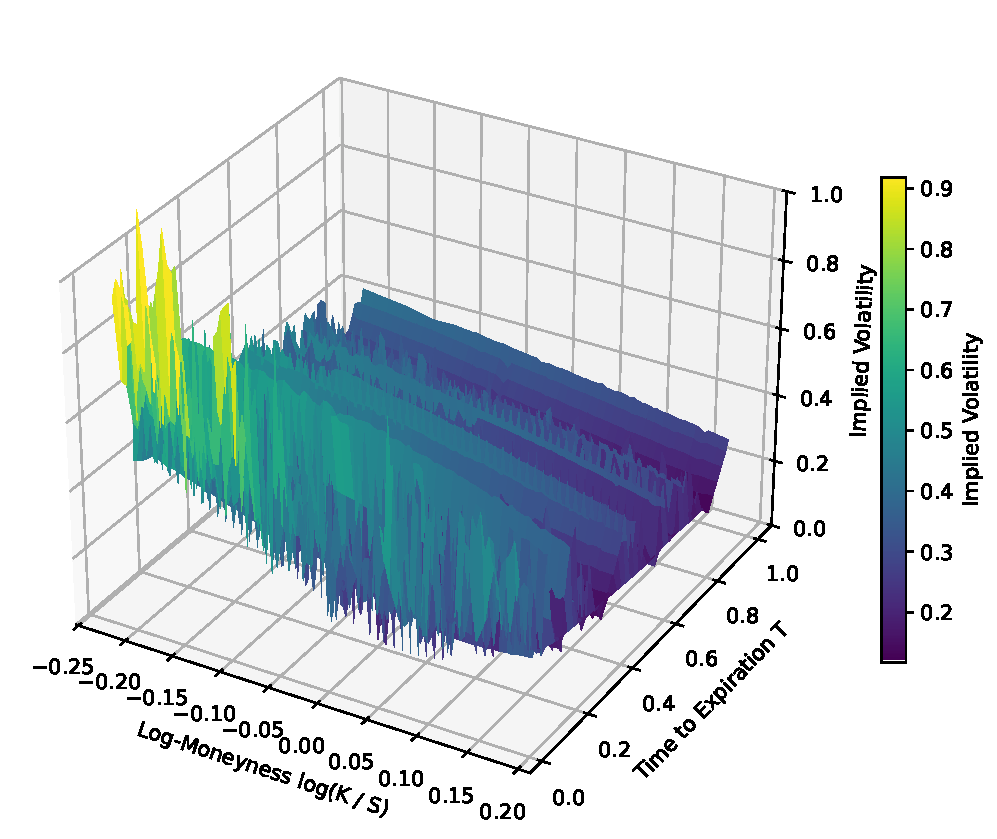
\includegraphics[width=\linewidth]{Images/implied_volatility_surface.pdf}

      \small Implied volatility surface
      \[
        \sigma_{\mathrm{imp}}(K,T)
      \]
    \end{column}

    \begin{column}{0.24\textwidth}
      \centering
      \Large
      \[
        \Longrightarrow
      \]
      \scriptsize
      \[
        \sigma_{\mathrm{loc}}^2(K,T)
        =
        \frac{\frac{\partial C}{\partial T}
        + rK\frac{\partial C}{\partial K}}
        {\frac{1}{2}K^2\frac{\partial^2 C}{\partial K^2}}
      \]
    \end{column}

    \begin{column}{0.38\textwidth}
      \centering
      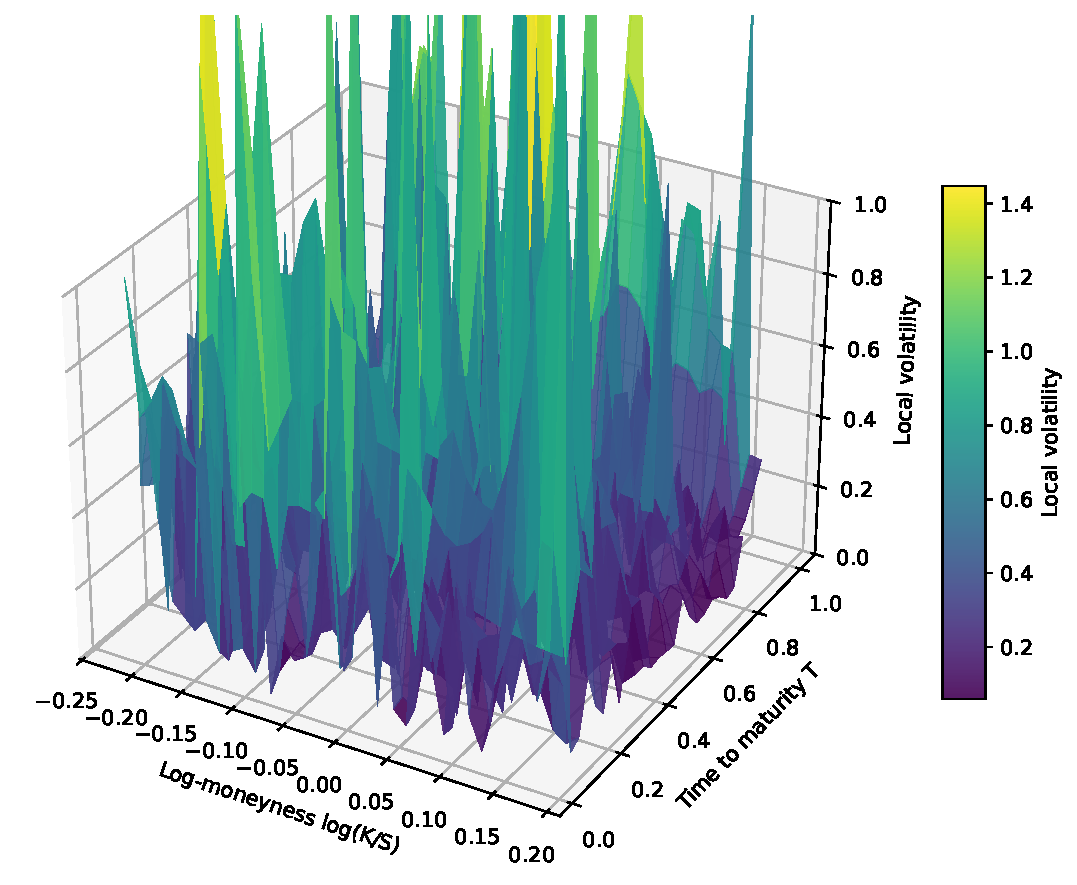
\includegraphics[width=\linewidth]{Images/local_volatility_surface.pdf}

      \small Local volatility surface
      \[
        \sigma_{\mathrm{loc}}(S,t)
      \]
    \end{column}
  \end{columns}
\end{frame}

\begin{frame}{Delta Proxy for Hedging}
  \begin{itemize}
    \item In reality
    \[
      \Delta_{\mathrm{Dupire}} = \frac{\partial C}{\partial S}.
    \]
    \item Where C is calculated from the local volatility PDE
    \item In our implementation, we use a proxy: look up
    $\sigma_{\mathrm{loc}}(S,t)$ and plug it into the Black--Scholes delta formula.
    \[
      \Delta_{\mathrm{proxy}}
      =
      N\!\left(
      \frac{\log(S/K) + \left(r+\frac{1}{2}\sigma_{\mathrm{loc}}^2\right)T}
      {\sigma_{\mathrm{loc}}\sqrt{T}}
      \right).
    \]
    \item This gives a fast hedge ratio for daily rebalancing.
    \item As a check: Dupire delta  $=0.47$ vs. proxy value delta $0.54$ for an ATM example.
  \end{itemize}
\end{frame}


%------------------------------------------------

\begin{frame}{Overview of Neural Network Approach}

\begin{center}
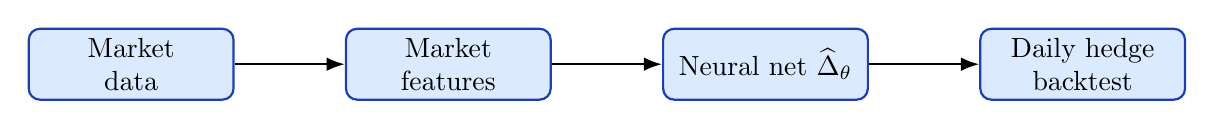
\begin{tikzpicture}[node distance=1.4cm, >=Latex]
  \tikzstyle{box}=[rectangle, rounded corners, draw=deepblue, fill=softblue, thick, minimum width=2.6cm, minimum height=0.9cm, align=center]
  \node[box] (data) {Market\\ data};
  \node[box, right=of data] (feat) {Market\\ features};
  \node[box, right=of feat] (nn) {Neural net $\widehat\Delta_\theta$};
  \node[box, right=of nn] (bt) {Daily hedge\\ backtest};
  \draw[->, thick] (data) -- (feat);
  \draw[->, thick] (feat) -- (nn);
  \draw[->, thick] (nn) -- (bt);
\end{tikzpicture}
\end{center}

\vspace{0.15cm}
\textbf{Note:} the network does \emph{not} predict stock returns / volatility. It directly predicts an option delta / hedge ratio.

\end{frame}
\begin{frame}{Learning Target: Realized Delta}
For an option contract observed on consecutive dates, the target is
\[
  y_i = \Delta^{\mathrm{real}}_i
  = \frac{C_{i+1}-C_i}{S_{i+1}-S_i},
\]
where $C_i$ is the option mid price and $S_i$ is the underlying price.

\vspace{0.25cm}
\begin{itemize}
  \item Group by the same contract: \texttt{expiration} and \texttt{strike}.
  \item Shift forward one row to compute next option and stock prices.
  \item Drop rows where $|S_{i+1}-S_i| < 0.01$.
  \item Clip the target to $[-2,2]$ to stabilize extreme ratios.
\end{itemize}

\end{frame}

%------------------------------------------------
\begin{frame}{Input Features}
Each training example is an option observation with a feature vector
\(
  x_i \in \mathbb{R}^{13}.
\)

\begin{columns}[T,onlytextwidth]
\begin{column}{0.48\textwidth}
\begin{block}{Option state}
\begin{itemize}
  \item moneyness
  \item log moneyness
  \item time to maturity $T$
  \item implied volatility
  \item Black--Scholes call delta
  \item mid price
  \item relative bid--ask spread
\end{itemize}
\end{block}
\end{column}
\begin{column}{0.48\textwidth}
\begin{block}{Market context}
\begin{itemize}
  \item 20-day realized volatility
  \item 60-day realized volatility
  \item volume
  \item open interest
  \item recent stock return
  \item recent absolute return
\end{itemize}
\end{block}
\end{column}
\end{columns}

\vspace{0.6cm}
\textbf{Role of Black--Scholes delta:} it is not the final answer; it is one informative input among many.
\end{frame}

%------------------------------------------------
\begin{frame}{Network Architecture}
The implemented model is a small feedforward neural network:
\[
\widehat\Delta_\theta(x)
= W_4\sigma\!\left(W_3\sigma\!\left(W_2\sigma\!\left(W_1x+b_1\right)+b_2\right)+b_3\right)+b_4,
\]
with ReLU activation $\sigma(z)=\max\{z,0\}$.

\vspace{0.2cm}
\begin{center}
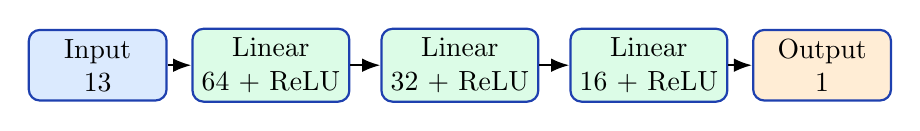
\begin{tikzpicture}[x=1cm,y=1cm, >=Latex]
  \tikzstyle{layer}=[rectangle, rounded corners, thick, draw=deepblue, fill=softblue, minimum width=1.75cm, minimum height=0.8cm, align=center]
  \node[layer] (in) at (0,0) {Input\\13};
  \node[layer, fill=softgreen] (h1) at (2.2,0) {Linear\\64 + ReLU};
  \node[layer, fill=softgreen] (h2) at (4.6,0) {Linear\\32 + ReLU};
  \node[layer, fill=softgreen] (h3) at (7.0,0) {Linear\\16 + ReLU};
  \node[layer, fill=softorange] (out) at (9.2,0) {Output\\1};
  \draw[->, thick] (in) -- (h1);
  \draw[->, thick] (h1) -- (h2);
  \draw[->, thick] (h2) -- (h3);
  \draw[->, thick] (h3) -- (out);
\end{tikzpicture}
\end{center}

\vspace{0.1cm}
The output is a scalar hedge ratio. At prediction time, it is clipped to $[-2,2]$.
\end{frame}

%------------------------------------------------
\begin{frame}{Training Objective}
The model is trained as a supervised regression problem:
\[
  \min_\theta \frac{1}{n}\sum_{i=1}^n
  \left(\widehat\Delta_\theta(x_i)-\Delta_i^{\mathrm{real}}\right)^2.
\]

\begin{itemize}
  \item Features are standardized by \texttt{StandardScaler}.
  \item Optimization uses Adam with learning rate $10^{-3}$.
  \item Default maximum training length: 300 epochs.
  \item Early stopping patience: 35 validation checks.
\end{itemize}

% \vspace{0.2cm}
% \begin{block}{Why MSE?}
% A wrong delta creates hedge error. Squared loss directly penalizes large deviations between predicted and realized hedge ratios.
% \end{block}
\end{frame}

%------------------------------------------------
\begin{frame}{Time-Split Design}
The code sorts the data by date and uses a chronological split:
\[
\underbrace{70\%}_{\text{train} }\quad
\underbrace{15\%}_{\text{validation} }\quad
\underbrace{15\%}_{\text{out-of-sample backtest} }.
\]

\vspace{0.3cm}
\begin{center}
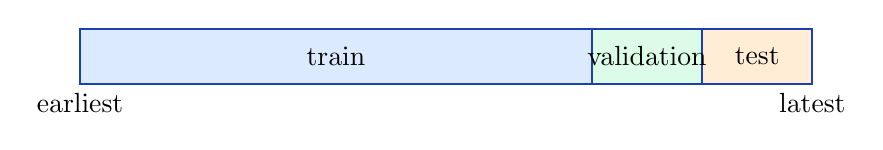
\begin{tikzpicture}
  \draw[fill=softblue, draw=deepblue, thick] (0,0) rectangle (6.5,0.7);
  \draw[fill=softgreen, draw=deepblue, thick] (6.5,0) rectangle (7.9,0.7);
  \draw[fill=softorange, draw=deepblue, thick] (7.9,0) rectangle (9.3,0.7);
  \node at (3.25,0.35) {train};
  \node at (7.2,0.35) {validation};
  \node at (8.6,0.35) {test};
  \node[below] at (0,0) {earliest};
  \node[below] at (9.3,0) {latest};
\end{tikzpicture}
\end{center}

\vspace{0.25cm}
\textbf{Reason:} financial time series should be evaluated forward in time, not by random shuffling.
\end{frame}

%------------------------------------------------
% \begin{frame}[fragile]{Core Code Pattern}
% \begin{lstlisting}[language=Python]
% class HedgeNet(nn.Module):
%     def __init__(self, input_dim):
%         super().__init__()
%         self.network = nn.Sequential(
%             nn.Linear(input_dim, 64), nn.ReLU(),
%             nn.Linear(64, 32), nn.ReLU(),
%             nn.Linear(32, 16), nn.ReLU(),
%             nn.Linear(16, 1),
%         )

%     def forward(self, x):
%         return self.network(x)
% \end{lstlisting}

% \vspace{0.15cm}
% This is deliberately simple: the project tests whether a compact MLP can improve hedge ratios, not whether a very deep model can overfit option data.
% \end{frame}

%------------------------------------------------
% \begin{frame}{How the NN Enters the Backtest}
% After training, the saved model and scaler are used to predict deltas on out-of-sample option rows:
% \[
%   \texttt{portfolio[``nn\_delta'']} = \widehat\Delta_\theta(x).
% \]

% \vspace{0.2cm}
% \begin{center}
% \begin{tikzpicture}[node distance=1.2cm, >=Latex]
%   \tikzstyle{box}=[rectangle, rounded corners, draw=deepblue, fill=softblue, thick, minimum width=2.6cm, minimum height=0.75cm, align=center]
%   \node[box] (portfolio) {Same option\\ portfolio};
%   \node[box, right=of portfolio, fill=softgreen] (dupire) {Dupire\\ delta};
%   \node[box, below=of dupire, fill=softorange] (nn) {NN\\ delta};
%   \node[box, right=1.4cm of $(dupire)!0.5!(nn)$, fill=softred] (metrics) {Compare\\ hedging metrics};
%   \draw[->, thick] (portfolio) -- (dupire);
%   \draw[->, thick] (portfolio) -- (nn);
%   \draw[->, thick] (dupire) -- (metrics);
%   \draw[->, thick] (nn) -- (metrics);
% \end{tikzpicture}
% \end{center}

% \vspace{0.1cm}
% The final comparison uses out-of-sample hedge performance, not in-sample training loss.
% \end{frame}

% %------------------------------------------------
% \begin{frame}{Evaluation Metrics}
% The NN hedge is compared with the Dupire hedge using portfolio-level and hedge-error metrics:
% \begin{itemize}
%   \item final value and total P\&L,
%   \item daily P\&L volatility and Sharpe ratio,
%   \item mean absolute hedging error,
%   \item RMSE hedging error,
%   \item maximum drawdown,
%   \item transaction costs and turnover.
% \end{itemize}

% \end{frame}

%------------------------------------------------

\begin{frame}{Conclusion}
    \begin{enumerate}
        \item Summary point one: Our educational exercise provides two comparable hedging strategies.
        
        \item Summary point two: This let's us delve into the standard metrics of a hedging strategy, visualize them and understand if one outperforms the other.
    \end{enumerate}
\end{frame}

\begin{frame}

\begin{figure}
    \centering
    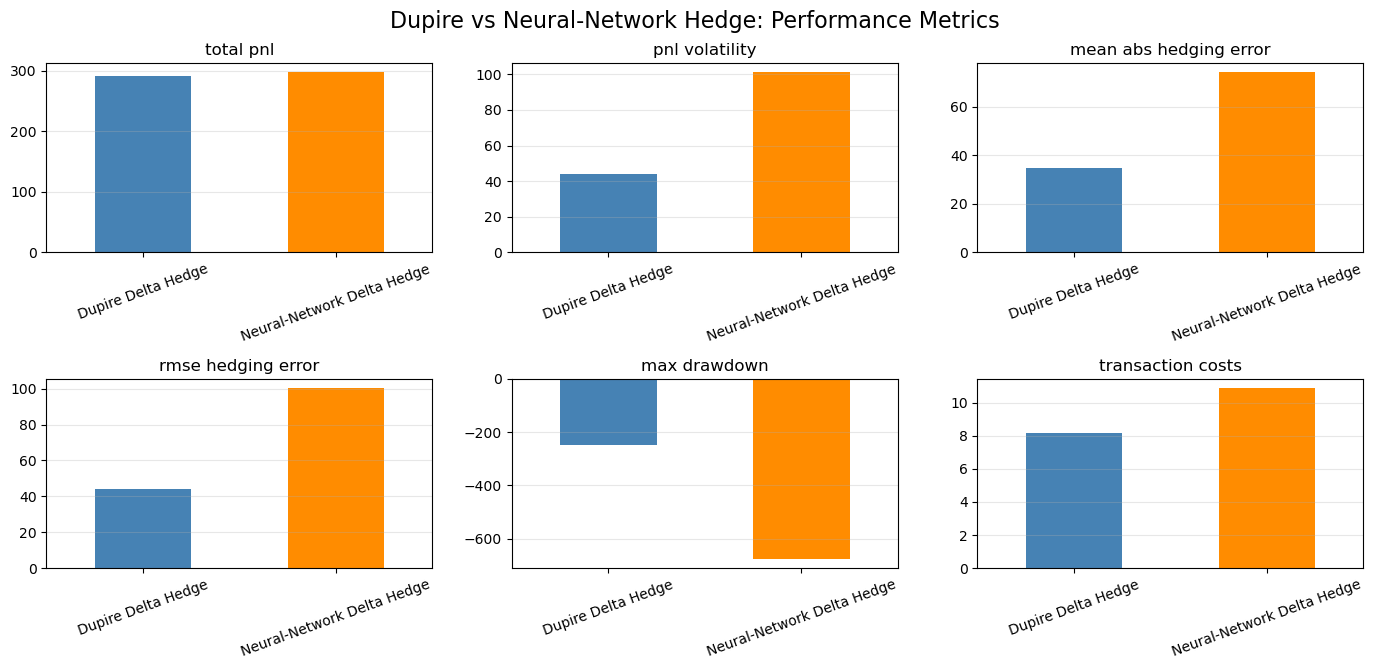
\includegraphics[width=1\linewidth]{Performance Metrics.png}

\end{figure}
\end{frame}


\begin{frame}

\begin{figure}
    \centering
    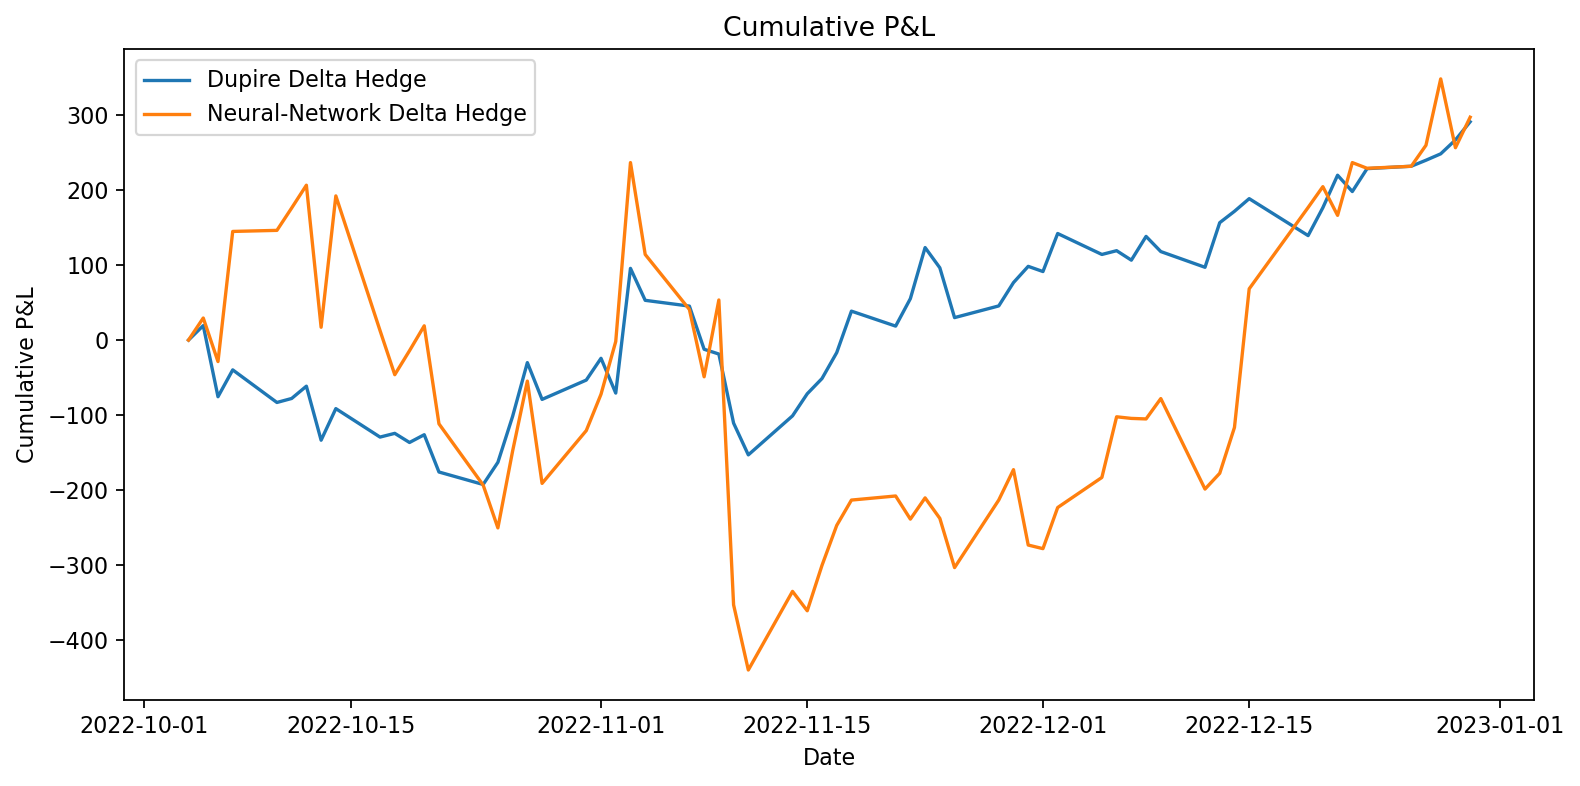
\includegraphics[width=1\linewidth]{Cumulative Profits & Losses.png}
\end{figure}
\end{frame}

\begin{frame}

\begin{figure}
    \centering
    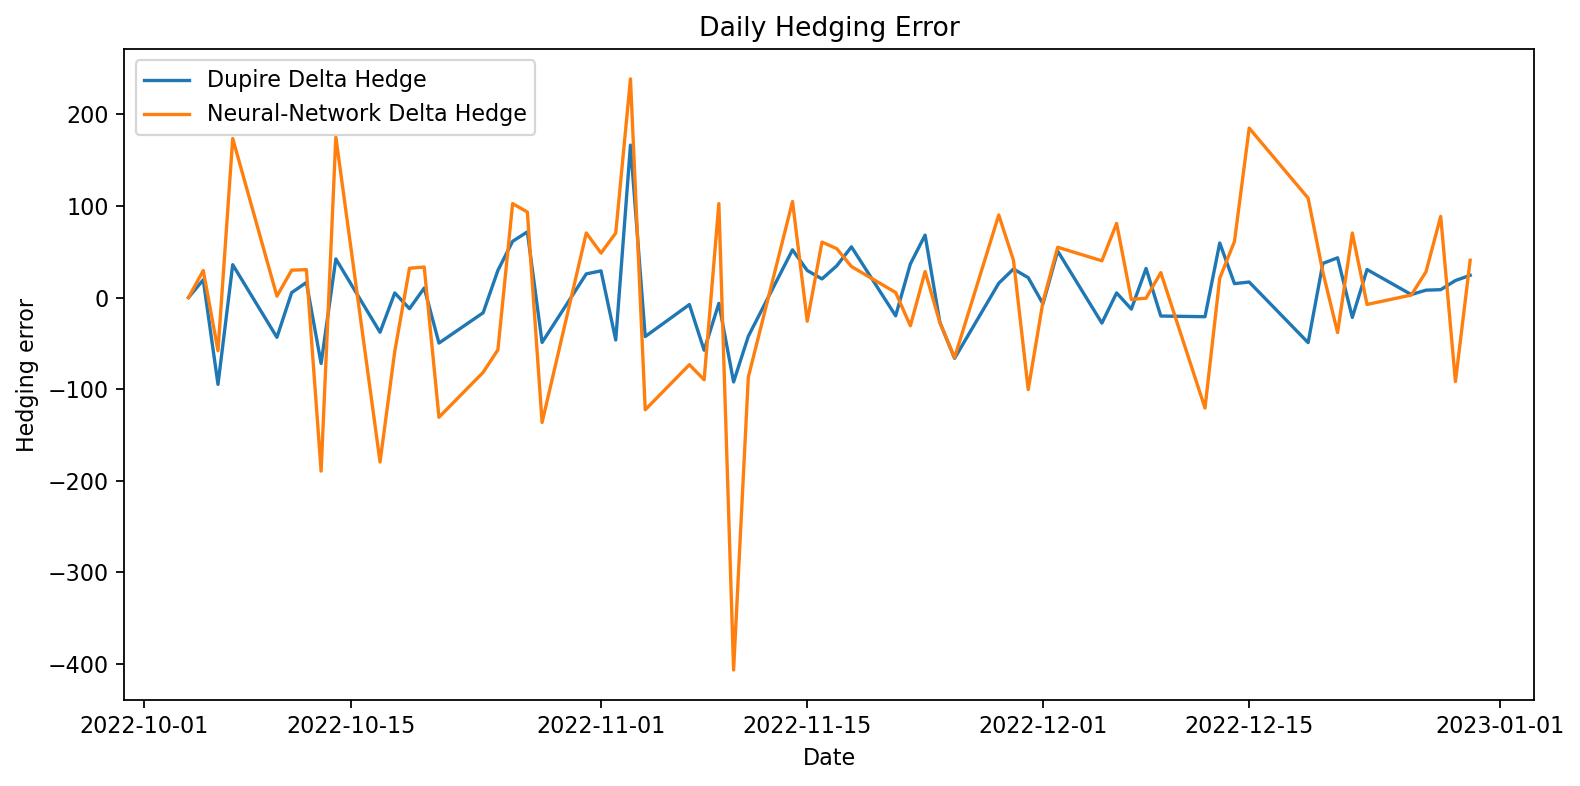
\includegraphics[width=1\linewidth]{Daily Hedging Error.png}
\end{figure}
\end{frame}

\begin{frame}

\begin{figure}
    \centering
    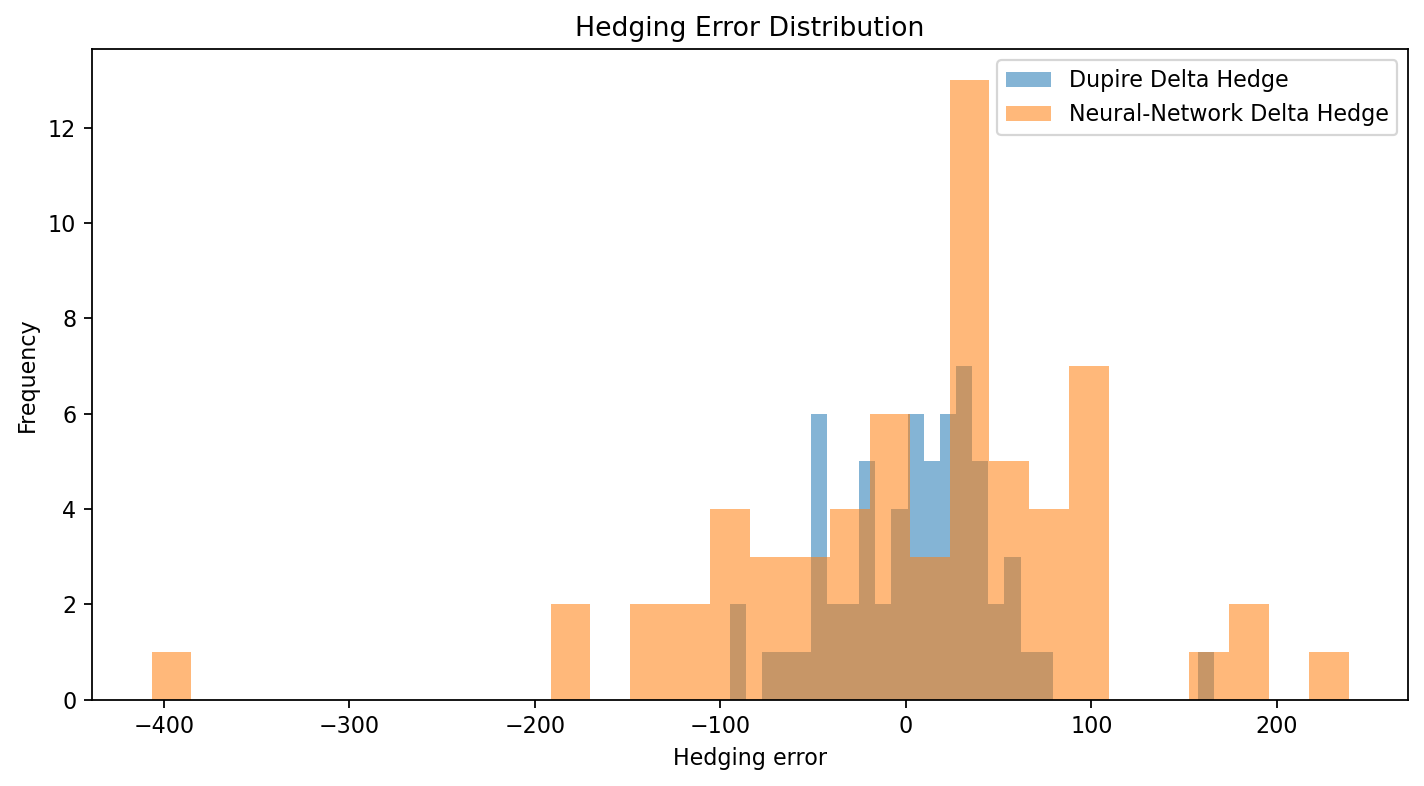
\includegraphics[width=1 \linewidth]{Hedging Error Distribution.png}

\end{figure}
\end{frame}

\begin{frame}

\begin{figure}
    \centering
    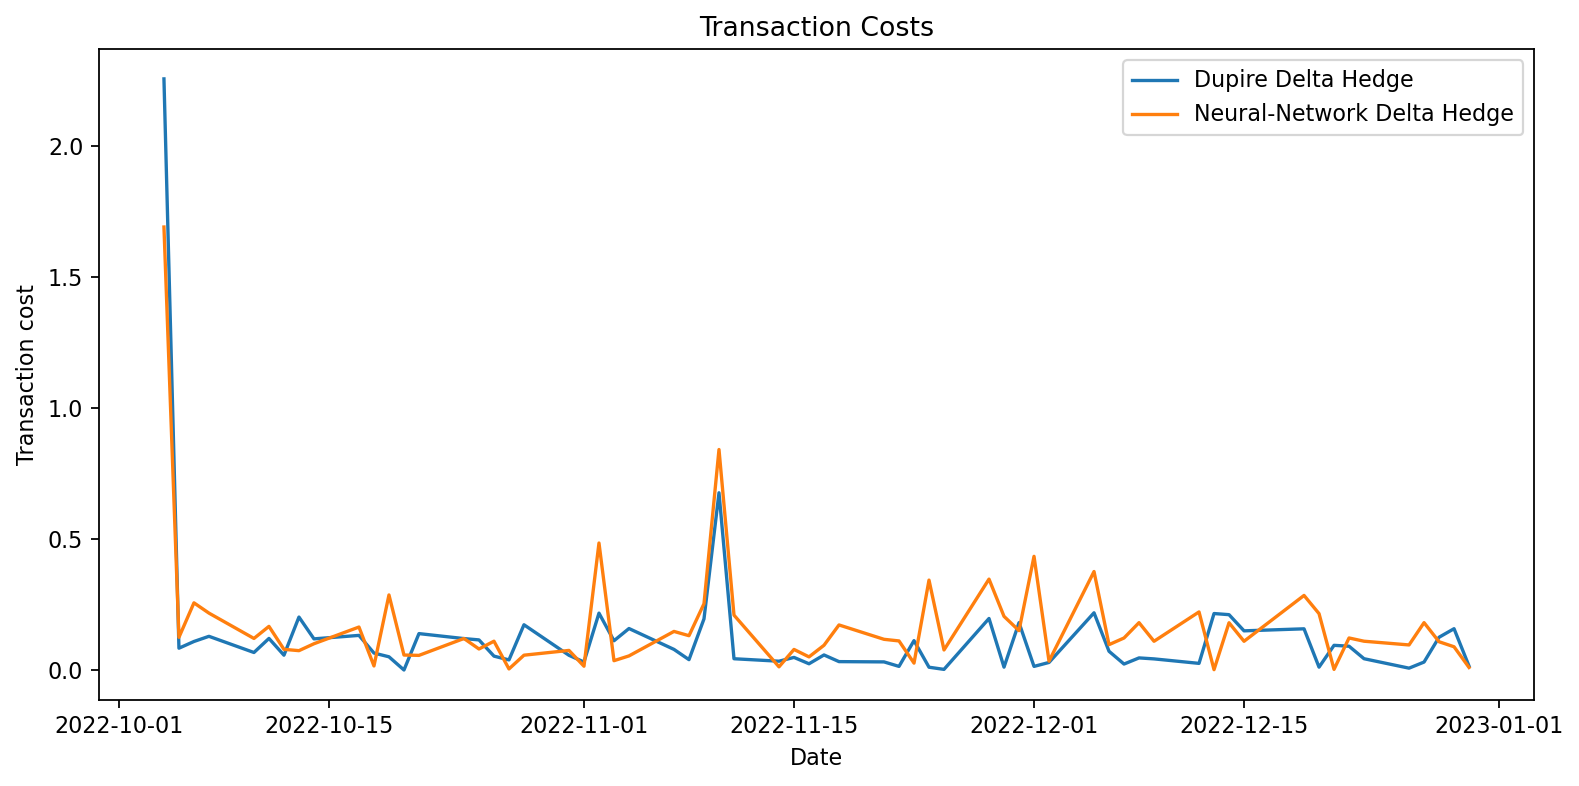
\includegraphics[width=1 \linewidth]{Transaction Costs.png}

\end{figure}
\end{frame}


\begin{frame}
\begin{block}{Final Takeaway}
Clearly the Dupire strategy outperformed the Neural Network strategy. Nonetheless, it actually provides evidence that developing hedging strategies that mix ideas from machine learning and traditional quantitative finance models is a natural step.
\end{block}
\end{frame}



% Thank you slide
\begin{frame}
    \centering
    \Huge Thank You!
    
    % \vspace{0.5cm}
    % \Large Questions?
\end{frame}


%------------------------------------------------
\end{document}
